\documentclass{article}
\usepackage{amsmath, amssymb, amsfonts, amsthm, mathtools}
\usepackage[utf8]{inputenc}
\usepackage[inline]{enumitem}
\usepackage{cancel}
\usepackage{soul}
\usepackage{hyperref}
\usepackage{tikz}
\newtheorem{theorem}{Theorem}
\newtheorem{lem}{Lemma}
\newtheorem{defn}{Definition}

\newcommand{\no}{\textbf{Choice required: {\color[rgb]{0, 0, 1} No.}}}
\newcommand{\yes}{\textbf{Choice required: {\color[rgb]{1, 0, 0} Yes.}}}
\newcommand{\thicc}{
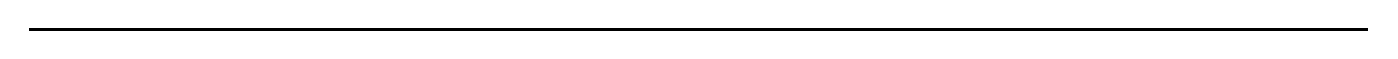
\begin{tikzpicture}
	\draw[very thick] (0, 0) -- (17, 0);
\end{tikzpicture}}
\newcommand{\dashed}{
\begin{tikzpicture}
	\draw[dashed] (0, 0) -- (17, 0);
\end{tikzpicture}}

\newcommand{\rng}{\operatorname{rng}}
\newcommand{\dom}{\operatorname{dom}}

\let\emptyset\varnothing
\setlength\parindent{0pt}

\usepackage{xcolor}
\definecolor{mybgcolor}{RGB}{50, 50, 50} %46, 51, 63

\usepackage{pagecolor}
% \pagecolor{mybgcolor}
% \color{white}

\usepackage{geometry}
\geometry{
    a4paper,
    total={170mm,257mm},
    left=20mm,
    top=20mm,
}

\title{Infinities and Beyond}
\author{Aryaman Maithani}
\date{January 28, 2020}

\begin{document}
\maketitle
\section{General results}

\begin{theorem}[Schr\"{o}der-Bernstein (SB)] \label{thm:sb} 
	If $\mathfrak{u}$ and $\mathfrak{v}$ are cardinal numbers such that $\mathfrak{u} \le \mathfrak{v}$ and $\mathfrak{v} \le \mathfrak{u},$ then $\mathfrak{u} = \mathfrak{v}.$	
\end{theorem}
\setcounter{theorem}{0}
Another way to phrase this is:
\begin{theorem}[Schr\"{o}der-Bernstein (SB)]
	If $U$ and $V$ are sets such that there's an injection from $U$ to $V$ and an injection from $V$ to $U,$ then there is a bijection from $U$ to $V$.
\end{theorem}
\no

\dashed

\begin{proof} 
	By hypothesis, there exist one-to-one functions $f:U\to V$ and $g:V\to U.$\\
	Define a function $\varphi:\mathcal{P}(U) \to \mathcal{P}(U)$ as follows:
	\begin{align} 
		\varphi(E) := U\setminus g[V\setminus f[E]] 
	\end{align}
	Now, we claim that if $E \subset F \subset U,$ then $\varphi(E) \subset \varphi(F).$\\
	Indeed, we have that $E \subset F \subset U \implies f[E] \subset f[F] \implies V\setminus f[F] \subset V\setminus f[E] \implies g[V\setminus f[F]] \subset g[V\setminus f[E]] \implies U\setminus g[V\setminus f[E]] \subset U\setminus g[V\setminus f[F]] \iff \varphi(E) \subset \varphi(F).$\\~\\
	Thus, we have
	\begin{align} 
		E \subset F \subset U \implies \varphi(E) \subset \varphi(F)
	\end{align}
	Define $\mathcal{D} := \{E \in \mathcal{P}(U) : E \subset \varphi(E)\}.$ Note that $\mathcal{D} \neq \emptyset$ as $\emptyset \in \mathcal{D}.$\\
	Define $D := \displaystyle\bigcup_{E \in \mathcal{D}}E.$\\
	Now, given any $E \in \mathcal{D},$ we have $E \subset D.$ By (2), this gives us that $\varphi(E) \subset \varphi(D).$ Also, by definition of $\mathcal{D},$ we have that $E \subset \varphi(E).$\\
	Thus, $E \subset \varphi(D)$ for all $E \in \mathcal{D}.$ It follows from the definition of $D$ that $D \subset \varphi(D).$ Applying (2) again gives us $\varphi(D) \subset \varphi(\varphi(D))$ and hence, $\varphi(D) \in \mathcal{D}.$ This now gives us that $\varphi(D) \subset D.$\\
	The inclusions in both directions give us that $\varphi(D) = D.$\\~\\
	For the sake of clarity, we can now see that we have arrived at the following result:\\
	There exist subsets $D \subset U$ and $R \subset V$ such that $f[D] = R$ and $g[V \setminus R] = U \setminus D.$ (Let this $D$ be the $D$ defined as earlier and let $R := f[D].$)\\
	We can now simply define the following bijection $h:U \to V$ as
	\begin{align*} 
		h(x) := \left\{\begin{array}{r l}
			f(x) & \text{ if }x \in D\\
			g^{-1}(x) & \text{ if }x \in U \setminus D 
		\end{array}
		\right.
	\end{align*}
	Note that $h$ indeed is well-defined as we have defined the value of $h$ for each $x$ uniquely. The fact that it is well-defined for $x \in U\setminus D$ follows from the fact that $g[V\setminus R] = U\setminus D$ and thus, every $x \in U \setminus D$ does have a pre-image. This is unique by the hypothesis that $g$ is one-to-one.\\
	The fact that $h$ is a bijection also follows from the properties of $D$ and $R.$
	\end{proof}

\thicc

\begin{theorem}[Comparing cardinalities]
	Let $U$ and $V$ be sets. Then either $|U| \le |V|$ or $|V| \le |U|.$
\end{theorem}
\yes

\dashed

\begin{proof}
	The idea will be to use Zorn's Lemma.\\
	Let $\mathcal{F}$ be the set of all one-to-one functions $f$ such that $\dom f \subset U$ and $\rng f \subset V.$ Note that $\mathcal{F} \neq \emptyset$ as $\emptyset \in \mathcal{F}.$\\
	We order $\mathcal{F}$ by inclusion. (Recall that every $f \in \mathcal{F}$ can regarded as a subset of $U \times V.$)\\
	Let $\mathcal{C} \subset \mathcal{F}$ be a chain in $\mathcal{F}.$ We show that $\mathcal{C}$ has an upper bound $u \in \mathcal{F}.$\\
	Define $u = \displaystyle\bigcup_{f \in \mathcal{C}}f.$\\
	One can straightaway observe that $\dom u = \displaystyle\bigcup_{f \in \mathcal{C}} \dom f \subset U$ and similarly, $\rng u \subset V.$\\
	Now, we show that given any $x \in \dom u,$ there a unique $y \in V$ such that $(x, y) \in u.$\\
	\textbf{Existence.} This is easy, for if $x \in \dom u,$ then $x \in \dom f$ for some $f \in \mathcal{C}$ and thus, $(x, f(x)) \in f \subset u.$\\
	\textbf{Uniqueness.} Suppose $(x, y_1)$ and $(x, y_2)$ belong to $u.$ We show that $y_1 = y_2.$\\
	$(x, y_1) \in u \implies \exists f_1 \in \mathcal{C} [(x, y_1) \in f_1].$\\
	$(x, y_2) \in u \implies \exists f_1 \in \mathcal{C} [(x, y_2) \in f_2].$\\
	As $\mathcal{C}$ is a chain, we have that $f_1 \subset f_2$ or $f_2 \subset f_1.$ WLOG, we assume that $f_1 \subset f_2.$ Thus, $(x, y_1) \in f_2.$\\
	However, $f_2$ is a function and thus, $y_1 = y_2,$ as desired.\\
	Thus, $u$ is indeed a function. \\
	Now we show that it is one-to-one as well. The argument is almost identical to what we gave for the uniqueness of $y.$ We assume that $(x_1, y)$ and $(x_2, y)$ belong to $u$ for some $y \in V$ and conclude that $x_1 = x_2.$\\
	Thus, $u \in \mathcal{F}.$ Now, it is easy to see that $u$ is an upper bound of $\mathcal{C}.$\\~\\
	Thus, by Zorn's Lemma, we get that there exists a maximal element $m \in \mathcal{F}.$\\
	\textbf{Claim.} Either $\dom m = U$ or $\rng m = V.$\\
	\emph{Proof.} Suppose not. Then $\dom m \neq U$ \emph{and} $\rng m \neq V.$ Thus, there exist $x \in U \setminus \dom m$ and $y \in V \setminus \rng m.$\\
	Thus, $(x, y) \notin m$ giving us $m \subsetneq m \cup \{(x, y)\}.$ However, $m \cup \{(x, y)\} \in \mathcal{F},$ contradicting the maximality of $m.$\\~\\
	If $\dom m = U,$ then $m$ is a one-to-one function from $U$ to $V$ giving us that $|U| \le |V|.$ Otherwise, $m^{-1}$ is a one-to-one function from $V$ to $U$ giving us that $|V| \le |U|.$

\end{proof}

\thicc

\begin{theorem}[Cantor]
	Let $U$ be a set. Then $|U| < |\mathcal{P}(U)|.$
\end{theorem}
\no

\dashed

\begin{proof}
	For $U = \emptyset,$ the statement is true as $\mathcal{P}(\emptyset) = \{\emptyset\}$ is a nonempty set and there is no surjective function from an empty set to a nonempty set. On the other hand, $\emptyset : \emptyset \to \{\emptyset\}$ is an injection.\\~\\
	Now we suppose that $U \neq \emptyset.$\\
	We first establish that $|U| \le |\mathcal{P}(U)|.$ Consider the map $i:U\to\mathcal{P}(U)$ defined as $x \overset{i}{\mapsto}\{x\}.$ It is easy to see that this is an injection for $\{x\} = \{y\} \iff x = y.$\\~\\
	Now, we show that $|U| \neq |\mathcal{P}(U)|.$ Suppose that there exists a bijection $h:U \to \mathcal{P}(U).$\\
	Define $S = \{x \in U : x \notin h(x)\}.$\\
	By definition, we have that $S \subset U$ and thus, $S \in \mathcal{P}(U).$\\
	By assumption, $h$ is a bijection and thus, there exists $x \in U$ such that $h(x) = S.$\\
	Now, by the law of excluded middle, either $x \in S$ or $x \notin S.$ We show that either leads to a contradiction.\\
	\textbf{Case 1.} $x \in S.$\\
	$x \in S \implies x \in h(x) \implies x \notin S,$ where the first implication is by the definition of $x$ and the second is by the definition of $S.$\\
	\textbf{Case 2.} $x \notin S.$\\
	$x \notin S \implies x \notin h(x) \implies x \in S,$ where the first implication is by the definition of $x$ and the second is by the definition of $S.$\\
	Thus, we get that $x \in S \iff x \notin S,$ a contradiction.
\end{proof}

\thicc
\begin{theorem}
	Every infinite set has a countably infinite subset.\\
	In other words, $|\mathbb{N}| \le |A|,$ if $A$ is infinite.
\end{theorem}
\yes

\dashed

\begin{proof}
	Let $A$ be a any infinite set.\\
	\textbf{Claim.} For any $n \in \mathbb{N},$ there exists a set $A_n \subset A$ such that $|A_n| = n.$\\
	\emph{Proof.} We prove this via induction. As $A \neq \emptyset,$ there exists $A_1 \subset A$ such that $|A_1| = 1.$\\
	Now, let $A_n \subset A$ be such that $|A_n| = n.$ If $A\setminus A_n$ were empty, then we would get that $A$ is finite. Thus, there exists $x \in A\setminus A_n.$ Letting $A_{n+1} = A_n \cup \{x\},$ we have $A_{n+1} \subset A$	and $|A_{n+1}| = n+1.$\\~\\
	Now, let $\{A_n\}_{n\in\mathbb{N}}$ be any such family of subsets of $A$ as described above. The existence of such a family is given by axiom of choice.\\
	For each $n \in \mathbb{N},$ define
	\[B_n = A_{2^n}\setminus\left(\bigcup_{k = 0}^{n-1}A_{2^k}\right).\]
	Given $n < m,$ we have that if $x \in B_n,$ then $x \in A_{2^n}$ but then $x \notin B_m.$ Thus the family $\{B_n\}_{n \in \mathbb{N}}$ is a pairwise disjoint family of subsets of $A,$ and for each $n \in \mathbb{N}$ we have
	\[|B_n| \ge 2^n - \sum_{k=0}^{n-1}2^k = 2^n - (2^n - 1) = 1.\]
	Thus, each $B_n$ is nonempty.\\
	Applying the axiom of choice to $\{B_n\}_{n\in\mathbb{N}}$ gives a choice function $f: \mathbb{N} \to \displaystyle\bigcup_{n\in \mathbb{N}}B_n\subset A$ such that $f(n) \in B_n$ for each $n \in \mathbb{N}.$ \\
	As the sets are pairwise disjoint, we have it that $f$ is one-to-one.\\
	Thus, $f[\mathbb{N}]$ is a countably infinite subset of $A.$
\end{proof}

\thicc

\begin{theorem}
	Any subset of a countable set is countable.
\end{theorem}
\no

\dashed

\begin{proof} 
	Let $A$ be a countable set and let $B \subset A.$ If $B$ is finite, then there is nothing to prove. Now, suppose that $B$ is infinite. Then, $A$ cannot be finite and thus, is countably infinite. Let $g$ be a bijection from $\mathbb{N}$ to $A.$ Let $a_n := g(n).$\\
	We now define a bijection $f:\mathbb{N} \to B$ as follows:\\
	$f(1) = a_{n_1}$ where $n_1$ is the smallest $n \in \mathbb{N}$ such that $a_n \in B;$ $f(k+1) = a_{n_{k+1}}$ where $n_{k+1}$ is the smallest $n \in \mathbb{N}$ such that $a_n \in B \setminus \{f(1), \ldots, f(k)\}.$\\~\\
	We now show that $f$ is a bijection.\\
	\textbf{One-to-one.} Let $n, m \in \mathbb{N}$ with $n \neq m.$ WLOG, $n < m.$\\
	Then, $f(m) \in B \setminus \{f(1), \ldots, f(n), \ldots, f(m-1)\}$ and thus $f(m) \neq f(n).$\\
	\textbf{Onto.} Let $x \in B.$ Then, $x = a_m$ for some $m \in \mathbb{N}.$\\
	Define $S = \{n \in \mathbb{N} : n < m, a_n \in B\}.$ Then we have $f(|S| + 1) = x.$
\end{proof}

\thicc

\begin{theorem} \label{thm:N2A}
	If $A$ is any nonvoid countable set, then there exists a surjective function $f : \mathbb{N} \to A.$
\end{theorem}
\no

\dashed

\begin{proof} 
	Since $A$ is countable, there exists a one-to-one function $g:A\to\mathbb{N}.$ Fix some $a \in A.$ Define $f:\mathbb{N}\to A$ as
	\[f(n) :=\left\{\begin{array}{c l}
		g^{-1}(n) & \text{ if } n \in \rng g\\
		a & \text{ if } n \notin \rng g
	\end{array}\right.\]
	Given any $x \in A,$ we have that $f(g(x)) = x.$ Thus, $f$ is surjective.
\end{proof}

\thicc
\begin{theorem} \label{thm:surjection}
	If $A$ and $B$ are two nonvoid sets and if there is a mapping $f$ from $A$ onto $B,$ then $|B| \le |A|,$ that is, there is a one-to-one map from $B$ to $A.$
\end{theorem}
\yes

\dashed

\begin{proof} 
	Let $g$ be a choice function function for the family $\{f^{-1}(b)\}_{b \in B}.$ Then $g$ is a one-to-one mapping from $B$ to $A.$ This follows from the fact that $b_1 \neq b_2 \implies f^{-1}(b_1)\cap f^{-1}(b_2) = \emptyset.$
\end{proof}

\thicc

\begin{theorem} 
	The union of any countable family of countable sets is a countable set, i.e., if $\{A_i\}_{i\in I}$ is a family of sets such that $I$ is a countable and each $A_i$ is countable, then $A = \displaystyle\bigcup_{i \in I}A_i$ is countable.
\end{theorem}
\yes

\dashed

\begin{proof} 
	Let $\{A_i\}_{i\in I}$ be as in the theorem. WLOG, we assume that $I$ is nonvoid and so is $A_i$ for each $i \in I.$ Applying Theorem \ref{thm:N2A} to obtain a surjection $g:\mathbb{N} \to I.$\\
	Now, note that for each $i \in I,$ there exists a surjective function $f_i : \mathbb{N} \to A_i.$\\
	Using the axiom of choice, we can fix one such surjection for each $i \in I.$\\
	Now, we define $h:\mathbb{N}\times\mathbb{N} \to A$ by $h(m, n) = f_{g(m)}(n).$ Then $h$ is a surjective function. By Theorem \ref{thm:surjection}, we get that $|A| \le |\mathbb{N}\times\mathbb{N}| = |\mathbb{N}|,$ where the last equality follows from Theorem \ref{thm:nn}.
\end{proof}

\thicc

\section{Cardinalities of specific sets}

\begin{theorem} \label{thm:nn} 
	$|\mathbb{N}\times\mathbb{N}| = |\mathbb{N}|$
\end{theorem}
\no 

\dashed

\begin{proof} 
	$(m, n) \mapsto 2^{m-1}(2n-1)$ is a bijection from $\mathbb{N}\times\mathbb{N}$ to $\mathbb{N}.$
\end{proof}

\thicc

\begin{theorem} \label{thm:qz}
	$|\mathbb{Z}| = |\mathbb{Q}| = |\mathbb{N}|$
\end{theorem}
\no

\dashed
\begin{proof} 
	$\mathbb{Z}$ and $\mathbb{Q}$ can both be written as a countable union of countable sets and thus, are countable. One can also avoid choice and appeal to \hyperref[thm:sb]{SB} by choosing suitable functions.
\end{proof}
\thicc 

\begin{theorem} \label{thm:2^n}
	$2^{\aleph_0} = \mathfrak{c}.$
\end{theorem}
\no

\dashed

\begin{proof}
	Let $A = \{0, 1\}^\mathbb{N}.$ Then, $|A| = 2^{\aleph_0}.$ Let $B = [0, 1).$ Then $|B| = \mathfrak{c}.$ Thus, it suffices to show that $|A| = |B|.$ We shall construct injections from $A$ to $B$ and vice-versa and then appeal to \hyperref[thm:sb]{SB}.\\~\\
	%
	$A \to B.$\\
	Define $f:A \to B$ as $f(\varphi) = \displaystyle\sum_{n=1}^{\infty}\dfrac{\varphi(n)}{3^n}.$\\
	This can be thought of as mapping an infinite sequence of $0$ and $1$ to the corresponding ternary number. As we don't have sequences with infinitely many trailing $2$s, it follows that $f$ is one-to-one.\\~\\
	%
	$B \to A.$\\
	Given any $x \in B,$ it has a unique binary representation if we don't allow trailing $1$s. Said formally, there is a unique representation of the form:
	\[x = \sum_{n=1}^{\infty}\frac{x_n}{2^n}\]
	where each $x_n$ is $0$ or $1$ and $x_n = 0$ for infinitely many $n \in \mathbb{N}.$\\
	Define $g:B \to A$ by $g(x) = \varphi_x$ where $\varphi_x:\mathbb{N}\to\{0, 1\}$ is defined as $\varphi_x(n) = x_n.$\\
	Thus, $g$ is a one-to-one mapping from $B$ to $A.$\\~\\
	%
	By \hyperref[thm:sb]{SB}, we are done.
\end{proof}

\thicc

\begin{theorem} \label{thm:r^n}
	$|\mathbb{R}^\mathbb{N}| = |\mathbb{R}|$ or $\mathfrak{c}^{\aleph_0} = \mathfrak{c}.$
\end{theorem}
\no

\dashed

\begin{proof} 
	By Theorem \ref{thm:2^n}, there exists a bijection $f:\mathbb{R}\to\{0, 1\}^\mathbb{N}.$ Given any $r \in \mathbb{R},$ let $f_r := f(r).$ That is, $f_r$ is a function from $\mathbb{N}$ to $\{0, 1\}$ for each $r \in \mathbb{R}.$\\~\\
	Now, given any sequence $(x_n)_{n \in \mathbb{N}} \in \mathbb{R}^\mathbb{N},$ we get a sequence of functions $(f_{x_n})_{n \in \mathbb{N}} \in (\{0, 1\}^\mathbb{N})^\mathbb{N}.$\\
	This sequence corresponds to a function $g : \mathbb{N}\times\mathbb{N} \to \{0, 1\}$ defined as $g(m, n) = f_{x_m}(n).$\\~\\
	It is easy to see the this correspondence is one-to-one. Thus, we get that
	\[|\mathbb{R}^\mathbb{N}| = |\{0, 1\}^{\mathbb{N}\times\mathbb{N}}| = |\{0, 1\}^\mathbb{N}| = |\mathbb{R}|.\]
	Note that we have used Theorem \ref{thm:nn}, that is $|\mathbb{N}\times\mathbb{N}| = |\mathbb{N}|.$
\end{proof}

\thicc

\begin{theorem} \label{thm:a^a}
	Let $\mathfrak{a}$ be an infinite cardinal number. Then $\mathfrak{a}^\mathfrak{a} = 2^\mathfrak{a}.$
\end{theorem}
\yes

\dashed

\begin{proof} 
	\[2^\mathfrak{a} \le \mathfrak{a}^\mathfrak{a} \le (2^\mathfrak{a})^\mathfrak{a} = 2^{\mathfrak{a}\cdot\mathfrak{a}} = 2^\mathfrak{a}.\]
\end{proof}

\emph{Remark.} Choice was used to conclude that $\mathfrak{a}\cdot\mathfrak{a} = \mathfrak{a}.$ However, there are cardinalities for which this is true even without choice. For them, the theorem holds even without choice. \\
In fact, $\mathfrak{a}\cdot\mathfrak{a} = \mathfrak{a}$ for all cardinalities implies $AC$.

\thicc

\begin{theorem} 
	Let $S$ be the set of continuous functions from $\mathbb{R}$ to $\mathbb{R}.$\\
	$|S| = \mathfrak{c}.$
\end{theorem}
\no 

\dashed

\begin{proof} 
	First, we show that $|S| \ge |\mathbb{R}|= \mathfrak{c}.$\\
	Note that given any $r \in \mathbb{R},$ the constant function $x \mapsto r$ belongs to $S.$ It is easy to see that this gives an injection $\mathbb{R} \xhookrightarrow{} S.$\\~\\
	Now, we show that $|S| \le |\mathbb{R}^\mathbb{N}| = |\mathbb{R}| = \mathfrak{c},$ where the equality $|\mathbb{R}^\mathbb{N}| = \mathfrak{c}$ follows from Theorem \ref{thm:r^n}.\\
	We know that $|\mathbb{Q}| = |\mathbb{N}|.$ Let $q : \mathbb{N} \to \mathbb{Q}$ be a bijection.\\
	Given any $f \in S,$ define the following sequence $(x_n) \in \mathbb{R}^\mathbb{N}$
	\[x_n = f(q(n)).\]
	Now, note that if two continuous functions agree at all rational points, then they must be equal. ($\because \mathbb{Q}$ is dense in $\mathbb{R}.$)\\
	Thus, the above mapping $f \mapsto (x_n)$ is an injection $S \xhookrightarrow{} \mathbb{R}^\mathbb{N}.$\\~\\
	By \hyperref[thm:sb]{SB}, we conclude that $|S| = \mathfrak{c}.$
\end{proof}

\thicc

\begin{theorem} 
	Let $S$ be the set of discontinuous functions from $\mathbb{R}$ to $\mathbb{R}.$\\
	$|S| = 2^\mathfrak{c}.$
\end{theorem}
\no 

\dashed

\begin{proof} 
	$S \subset \mathbb{R}^\mathbb{R}$ and thus, $|S| \le |\mathbb{R}^\mathbb{R}| = 2^\mathfrak{c}.$ (Theorem \ref{thm:a^a}.)\\~\\
	Now, we show that $|S| \ge 2^\mathfrak{c}.$\\
	We create a injection from $\mathcal{P}(\mathbb{R}) \setminus \{\emptyset, \mathbb{R}\}$ to $S.$\\
	Let $A \in \mathcal{P}(\mathbb{R}) \setminus \{\emptyset, \mathbb{R}\}.$ Define $\varphi(A) = \chi_A,$ the indicator function of $A \subset \mathbb{R}.$\\
	It is easy to see that $\chi_A$ is discontinuous. This follows from the fact that $A = \chi_A^{-1}(\{1\})$ and $\mathbb{R}\setminus A = \chi_A^{-1}(\{0\})$ would have to be open subsets of $\mathbb{R},$ if $\chi_A$ were continuous but $\mathbb{R}$ is connected, so this is not possible. ($\because A \notin \{\emptyset, \mathbb{R}\}.$)\\~\\
	As $|\mathcal{P}(\mathbb{R}) \setminus \{\emptyset, \mathbb{R}\}| = |\mathcal{P}(\mathbb{R})| = 2^\mathfrak{c},$ the result follows from \hyperref[thm:sb]{SB}.
\end{proof}

\thicc 

\begin{theorem} 
	Let $S$ be the set of continuous functions from $\mathbb{Q}$ to $\mathbb{Q}.$\\
	$|S| = \mathfrak{c}.$
\end{theorem}
\no 

\dashed

\begin{proof} 
	First, we show that $|S| \le \mathfrak{c}.$\\
	Note that $S \subset \mathbb{Q}^\mathbb{Q}$ and thus $|S| \le |\mathbb{Q}^\mathbb{Q}| = \aleph_0^{\aleph_0} = 2^{\aleph_0}=\mathfrak{c}.$ (Theorems \ref{thm:qz}, \ref{thm:a^a}, and \ref{thm:2^n}.)\\~\\
	Now, we show that $|S| \ge |\mathbb{N}^\mathbb{N}| = |\mathbb{R}| = \mathfrak{c}.$\\
	Let $f \in \mathbb{N}^\mathbb{N}$ be given. Using this, we create a function $\varphi_f:\mathbb{Q} \to \mathbb{Q}$ as follows:\\
	$\varphi_f(x) = f(1)$ for all $x < 1,$
	$\varphi_f(n) = f(n)$ for all $n \in \mathbb{N},$\\
	for $x \in \mathbb{Q}\setminus\mathbb{N}$ and $x > 1,$ let $p = \lfloor x\rfloor$ and define $\varphi_f(x) = (x - p)(f(p+1) - f(p)) + f(p).$\\~\\
	It is easy to show that $\varphi_f \in S$ and $f \neq g \implies \varphi_f \neq \varphi_g$ as $\varphi_f$ agrees with $f$ at all naturals.\\
	($\varphi_f$ is the functions obtained by joining the points of the graph of $f.$)\\~\\
	The result now follows from \hyperref[thm:sb]{SB}.
\end{proof}

\thicc

\begin{theorem} 
	Let $S$ be the set of discontinuous functions from $\mathbb{Q}$ to $\mathbb{Q}.$\\
	$|S| = \mathfrak{c}.$
\end{theorem}
\no 

\dashed

\begin{proof} 
	First, we show that $|S| \le \mathfrak{c}.$\\
	Note that $S \subset \mathbb{Q}^\mathbb{Q}$ and thus $|S| \le |\mathbb{Q}^\mathbb{Q}| = \aleph_0^{\aleph_0} = 2^{\aleph_0}=\mathfrak{c}.$ (Theorems \ref{thm:qz}, \ref{thm:a^a}, and \ref{thm:2^n}.)\\~\\
	Now, we show that $|S| \ge |\mathbb{N}^\mathbb{N}| = |\mathbb{R}| = \mathfrak{c}.$\\
	Let $f \in \mathbb{N}^\mathbb{N}$ be given. Using this, we create a function $\varphi_f:\mathbb{Q} \to \mathbb{Q}$ as follows:\\
	\[\varphi_f(x) = \left\{\begin{array}{rl}
		f(x) & \text{ if } x \in \mathbb{N}\\
		0 & \text{ if } x \notin \mathbb{N}
	\end{array}
	\right.\]
	It is easy to show that $\varphi_f \in S$ and $f \neq g \implies \varphi_f \neq \varphi_g$ as $\varphi_f$ agrees with $f$ at all naturals.\\~\\
	The result now follows from \hyperref[thm:sb]{SB}.
\end{proof}

\thicc

\begin{theorem} 
	$|\mathbb{N}^\mathbb{R}| = |2^\mathbb{R}|$ or $\aleph_0^\mathfrak{c} = 2^\mathfrak{c}.$
\end{theorem}
\no 

\dashed

\begin{proof} 
	\[|2^\mathbb{R}| \le |\mathbb{N}^\mathbb{R}| \le |\mathbb{R}^\mathbb{R}| = |2^\mathbb{R}|.\]
\end{proof}

\thicc

\begin{theorem} 
	Let $\mathfrak{a} \ge \aleph_0.$ Then, $\mathfrak{a}! = 2^\mathfrak{a}.$
\end{theorem}
\yes

\begin{proof} 
	Let $A$ be a set with cardinality $\mathfrak{a}$ and let $S$ be the set of all bijections from $A$ to itself. By definition, we have $|S| = \mathfrak{a}!.$\\~\\
	Note that we have $|S| \le |A^A| = 2^\mathfrak{a}.$ (Theorem \ref{thm:a^a}.)\\
	Now we show that $|S| \ge |\mathcal{P}(A)| = 2^\mathfrak{a}.$\\
	If $A$ is infinite, then we have that $|A| = |A \times \{0, 1\}|.$ (This uses choice.)\\
	Thus, it suffices to show that there are as many bijections from $A \times \{0, 1\}$ as there are elements in $\mathcal{P}(A).$\\
	Let $B \in \mathcal{P}(A).$ Define the following function $f_B : A\times \{0, 1\} \to A \times \{0, 1\}.$\\
	\[f_B\left((a, x)\right) = \left\{\begin{array}{rl}
		(a, 0) & \text{ if } a \notin B \text{ and } x = 0\\
		(a, 1) & \text{ if } a \notin B \text{ and } x = 1\\
		(a, 0) & \text{ if } a \in B \text{ and } x = 1\\
		(a, 1) & \text{ if } a \in B \text{ and } x = 0\\
	\end{array}
	\right.\]
	That is, $f_B$ fixes all elements of the form $(a, 0)$ and $(a, 1)$ if $a \notin B$ and swaps them otherwise.\\
	It is clear that $B \mapsto f_B$ is an injection from $\mathcal{P}(A)$ to $S$ and thus, we are done by \hyperref[thm:sb]{SB}.
\end{proof}

\section{Summary}
\begin{enumerate} 
	\item $|2^\mathbb{N}| = |\mathbb{R}|.$
	\item $|\mathbb{R}^\mathbb{N}| = |\mathbb{R}|.$
	\item $|\mathbb{N}^\mathbb{R}| = |2^\mathbb{R}|.$
	\item $|C(\mathbb{R}, \mathbb{R})| = |\mathbb{R}|.$
	\item $|C(\mathbb{Q}, \mathbb{Q})| = |\mathbb{R}|.$
	\item $|X^X| = 2^{|X|}.$ (C)
	\item $|X|! = 2^{|X|}$ if $|X| = \infty.$ (C)
\end{enumerate}
\end{document}